\chapter{La piattaforma robot}
%\vspace{0.5cm}

\label{cha:789}
EvoBot è un robot che unisce elementi delle stampanti 3D con quelli della robotica modulare per fornire a chimici, microbiologi e ricercatori nel campo della vita (a livello chimico) artificiale, uno strumento economico ed estendibile basato su una piattaforma open source di robotica per il trattamento di liquidi. La particolarità di EvoBot sta nell'interazione continua ed in tempo reale dell'utente con l'esperimento in corso.\cite{introd-robot} Inoltre utilizzare un robot per la gestione degli esperimenti ci ha permesso di diminuire, quasi annullare, l'incertezza e la variazione tra gli esperimenti causata dalla mano umana. 
\\Come le comuni stampanti 3D,  questo robot è composto da una componente hardware guidata da una parte software. 

\section{La componente hardware}
EvoBot è composto, a livello elettronico, da un Arduino Mega 2560 su cui è montata una scheda RAMPS (RepRap Arduino Mega Pololu Shield); queste due schede controllano la testa del robot, i moduli ad essa collegati e gli input provenienti da sensori esterni. 
A livello meccanico, invece, è strutturato in tre strati: \emph{actuation layer}, \emph{experimental layer} e  \emph{observation layer}.
\\Partendo dal basso si trova lo strato dell'osservazione: \emph{observation layer}. Questo \emph{layer} non prevede nessuna interazione con gli esperimenti in corso sul layer superiore. E' utilizzato per il posizionamento di moduli che andranno a raccogliere dati, senza manipolare direttamente l'esperimento, che verranno forniti sia al robot sia all'utente. Nel nostro caso è presente una webcam. 
	\begin{figure}[h]
	  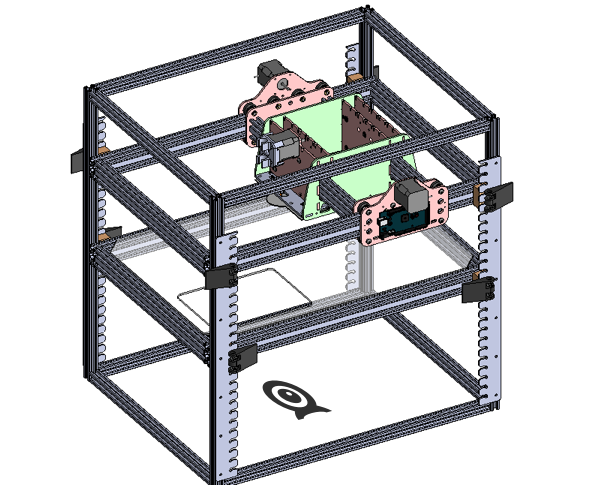
\includegraphics[scale=0.40]{immagini/observational-layer.png}
	\centering
	 \caption{La struttura completa con l'observational layer}
	\end{figure} 

\pagebreak
Il secondo strato è quello degli esperimenti: \emph{experimental layer}. Questo strato è essenzialmente composto da una cornice in alluminio, identica a quella della struttura esterna del robot, che racchiude una piastra di vetro. Su questo strato possono essere posti i recipienti richiesti dagli specifici esperimenti. Una fessura rettangolare ad uno degli angoli permette le manovre di sostituzione dei recipienti in uso. La sua funzionalità verrà sfruttata in futuro creando un distributore automatico di  \emph{Petri dish} da posizionarvi all'interno.
	\begin{figure}[h]
	  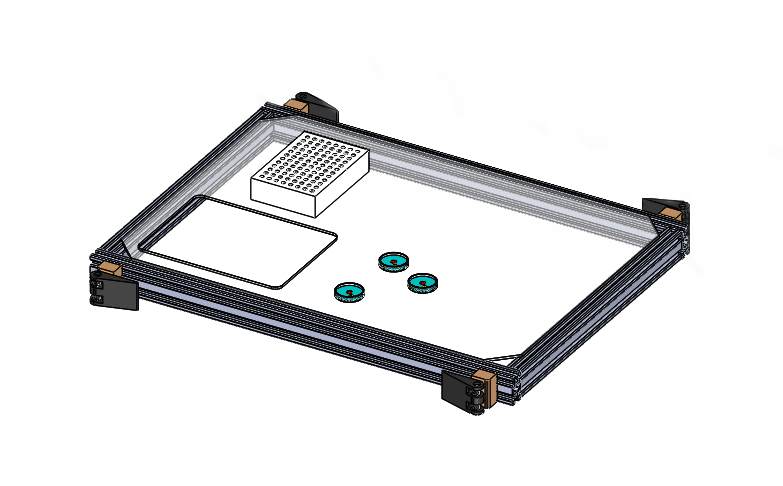
\includegraphics[scale=0.40]{immagini/experiment_layer.png}
		\centering 
	\caption{experimental layer}
	\end{figure} 
\\L'ultimo dei tre strati è lo strato di attivazione, \emph{actuation layer}, ovvero la testa del robot.  Questo layer si occupa del movimento della testa sul piano orizzontale per mezzo di un meccanismo cinghia-ruota dentata con due motori \emph{stepper}. La testa si può muovere nelle due direzioni sul livello orizzontale: \emph{x} e \emph{z}.

	\begin{figure}[h]
	  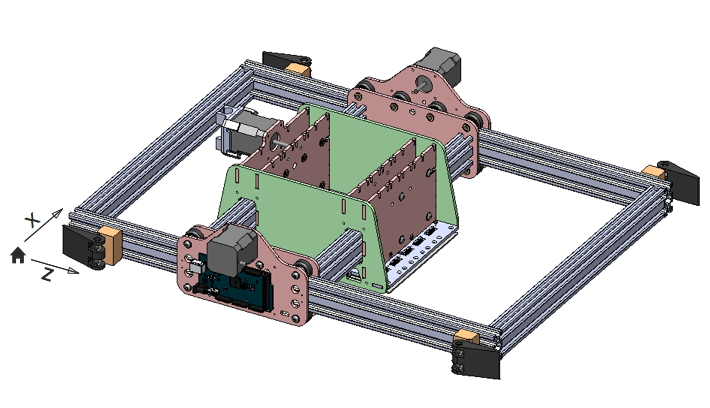
\includegraphics[scale=0.30]{immagini/actuation_layer.png}
		\centering	
	 \caption{actuation layer}
	\end{figure}
\pagebreak

\subsection{La testa}
La \emph{head}, testa del robot, è la componente principale dell'\emph{actuation layer}. E' composta di 17 \emph{socket} all'interno delle quali possono essere inseriti diversi moduli. Tuttavia, per come è stata strutturata, non c'è possibilità di inserire tutti i moduli contemporaneamente. Essa può contenere fino ad un massimo di 11 moduli per fornire funzionalità differenti. Ad oggi esiste soltanto il modulo siringa ma si prevede nel breve futuro, la costruzione di altri moduli come sensori di pH e di temperatura. 
	\begin{figure}[h]
	\centering
   		{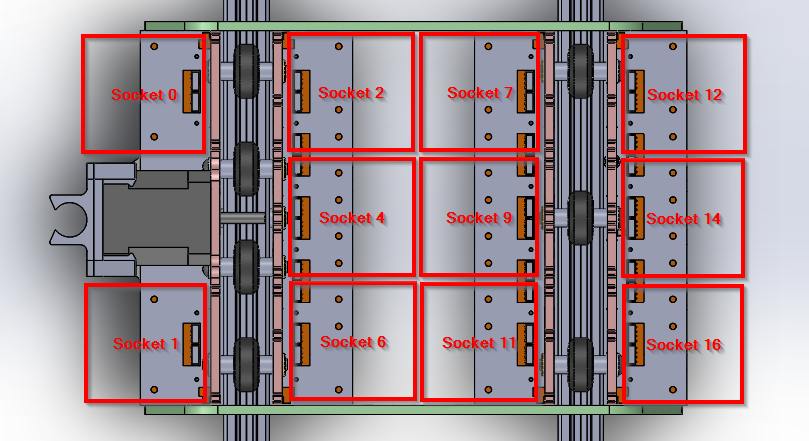
\includegraphics[width=8cm]{immagini/head_sockets_1.png}}
 	\hspace{5mm}
   		{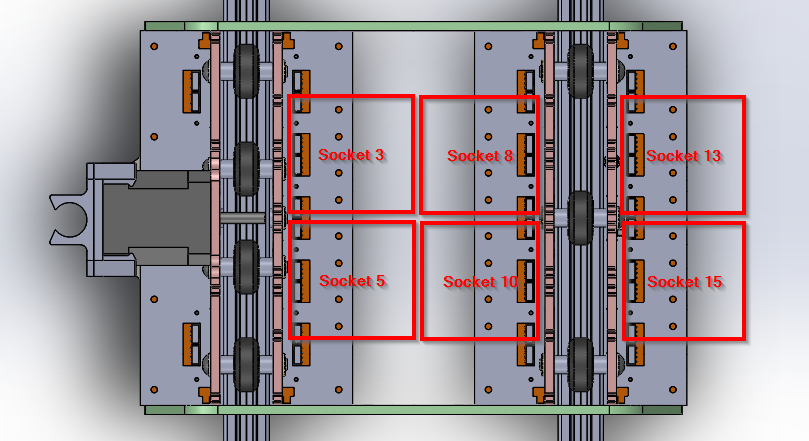
\includegraphics[width=8cm]{immagini/head_sockets.png}}
	\caption{socket disposition}
 	\end{figure}


\subsection{Le siringhe}
\label{sec:01456}
Il modulo siringa ha due gradi di movimento verticale. Ogni modulo è composto di un motore passo-passo lineare per il movimento dello stantuffo, \emph{plunger}, e di un meccanismo a rocchetto e cremagliera con un secondo motore passo-passo per il movimento del corpo della siringa. La siringa può essere facilmente sostituita dando all'utente l'opportunità di utilizzare siringhe con specifiche differenti in base alle necessità dell'esperimento. Le siringhe sono la componente di EvoBot che gli consente di gestire sostanze liquide.
	\begin{figure}[h]
	  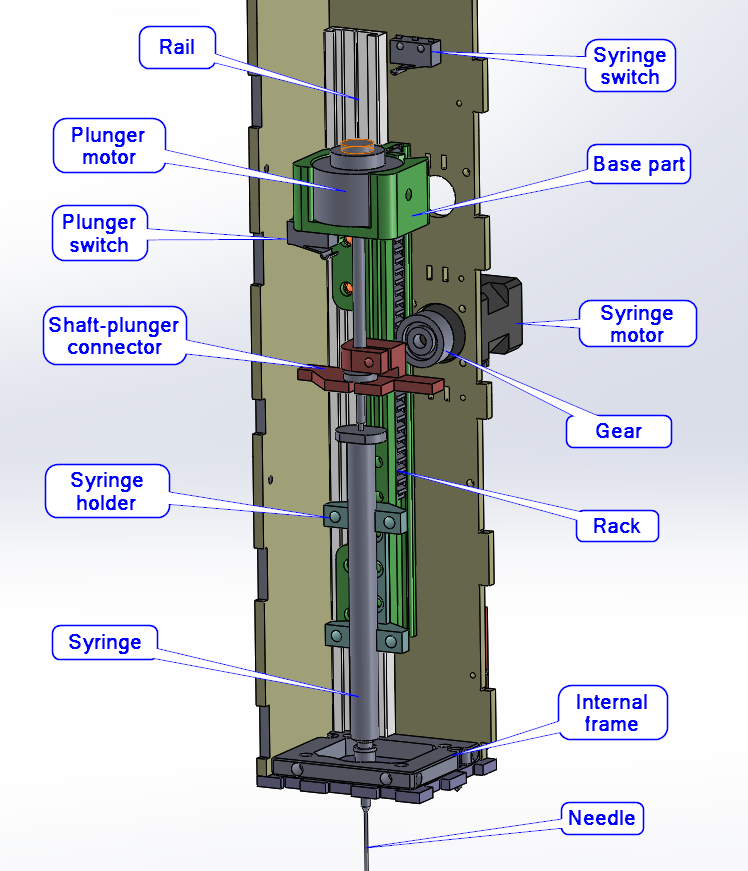
\includegraphics[scale=0.30]{immagini/syringe_parts.png}
		\centering
	 \caption{syringe module}
	\end{figure} 

\pagebreak 
\section{La componente software}
\label{sec:123}
La finalità della componente software è quella di fornire all'utente finale un'interfaccia facilmente programmabile per guidare il robot. Il software è suddiviso in una \emph{host side} e in una \emph{robot side}. La prima comunica con la seconda attraverso una connessione USB. La \emph{robot side} è una versione modificata del firmware Marlin usato nei programmi opensource delle stampanti 3D. 
\\Il linguaggio di programmazione utilizzato per la stesura delle API e dei programmi successivi è Python. La suite software offerta al momento dell'installazione è composta da tre elementi:
un programma di \emph{computer vision} per la calibrazione del robot, un'interfaccia grafica per il controllo manuale del robot ed un esempio di programma, sviluppato utilizzando le API, per l'identificazione delle componenti di uno specifico esperimento.
\\L'obiettivo dello sviluppo della componente software è stato quello di creare un programma in grado di controllare il robot manualmente in tempo reale e raccogliere i dati necessari dagli esperimenti eseguiti, di cui si parlerà nel prossimo capitolo. 

\subsection{Il controllo manuale}
\label{sec:00123}
La scelta di un software per il controllo manuale del robot nasce dalla necessità di ottenere la posizione di oggetti di interesse (Petri dishes e recipienti vari) sullo strato degli esperimenti. L'interfaccia grafica permette di testare le diverse funzioni del robot senza il bisogno di ricorrere alla programmazione. Per esempio, si può muovere la testa del robot fino a centrare uno dei contenitori, far scendere la siringa all'interno di questo e registrare la posizione del centroide dell'oggetto. 
\\Per controllare manualmente EvoBot si utilizza Printrun \cite{printrun}, una \emph{3D printing host suite}  opensource, con la quale, attraverso dei codici G standard, si controlla il movimento della testa del robot e con dei codici M speciali si controlla il movimento delle siringhe e degli stantuffi. Inoltre con i codici M si possono identificare i limiti dei due movimenti che una siringa può compiere.

\subsection{La calibrazione}
\label{sec:01123}
La calibrazione è il primo passo importante per correlare il sistema di coordinate della videocamera con quello del robot. A questo scopo viene creata la matrice di trasformazione compiendo le istruzioni imposte dal programma calibrationExample.py. 
Avendo la possibilità di posizionare le differenti piastre di Petri su tutto lo strato degli esperimenti o di impostare la distanza tra \emph{l'actuation layer} e \emph{experimental layer}, il programma è pensato per specificare i punti esatti per una massima accuratezza nella calibrazione. All'interno del programma si definisce il punto in cui è posizionata la Petri \emph{dish}, il suo diametro e la distanza tra i due layer.
Avvenuta la calibrazione, si hanno a disposizione le matrici di ogni siringa da poter utilizzare nei programmi successivi per muovere le siringhe nei punti richiesti dagli esperimenti.

\subsection{L'identificazione delle droplet}
\label{sec:02123}
Una delle finalità prioritarie del progetto è l'identificazione di gocce, \emph{droplet}, per trovare l'area, il colore, il numero, la forma e, più importante, per tracciarne il movimento.
%Come spiegato nella sezione 1.2.1le droplet.... aggiungere minchiate

La componente principale utilizzata per l'identificazione è la libreria OpenCV (Open Source Computer Vision Library)\cite{opencv} che include diverse funzioni ed algoritmi di \emph{computer vision}. 











 

